\documentclass{beamer}

\usepackage[T1]{fontenc}
\usepackage{lmodern}
\usepackage{graphicx}
\usepackage{amsmath}
\usepackage{amssymb}
\usepackage{booktabs}
\usepackage{xcolor}
\usepackage{tikz}
\usepackage{array}
\usepackage{colortbl}
\usepackage[authoryear,round]{natbib}
\usepackage{ragged2e}

\usetheme{Madrid}
\usecolortheme{default}
\setbeamertemplate{navigation symbols}{}
\setbeamertemplate{footline}[frame number]
\setbeamersize{text margin left=0.6cm, text margin right=0.6cm}

\definecolor{myprimary}{HTML}{FF9D00}
\definecolor{mysecondary}{HTML}{FF8360}
\definecolor{mydark}{HTML}{243447}
\definecolor{mylight}{HTML}{FFF4E8}
\definecolor{mysoft}{HTML}{F7F7F7}

\setbeamercolor{structure}{fg=myprimary}
\setbeamercolor{title}{fg=white,bg=myprimary}
\setbeamercolor{subtitle}{fg=myprimary}
\setbeamercolor{frametitle}{fg=white,bg=myprimary!90}
\setbeamercolor{block title}{fg=white,bg=myprimary!85}
\setbeamercolor{block body}{fg=black,bg=mylight}
\setbeamercolor{normal text}{fg=mydark,bg=white}
\setbeamercolor{alerted text}{fg=mysecondary}

\setbeamerfont{title}{series=\bfseries,size=\Large}
\setbeamerfont{frametitle}{series=\bfseries,size=\large}
\setbeamerfont{block title}{series=\bfseries}
\setbeamertemplate{bibliography item}[text]
\setlength{\bibsep}{1pt plus 0.2ex}
\bibliographystyle{abbrvnat}

\newcommand{\lerobot}{\texttt{lerobot}}
\newcommand{\lerobotdataset}{\texttt{LeRobotDataset}}
\newcommand{\pizero}{\(\pi_0\)}
\newcommand{\highlight}[1]{\textcolor{myprimary}{\textbf{#1}}}
\newcommand{\statbox}[2]{%
  \begingroup
  \setlength{\fboxsep}{8pt}%
  \colorbox{mylight}{\parbox{\dimexpr\linewidth-2\fboxsep\relax}{\raggedright\textbf{\large #1}\\[-1pt]\small #2}}%
  \endgroup
}

\newcommand{\circled}[1]{%
  \tikz[baseline=(char.base)]\node[draw,circle,inner sep=1pt,thick](char){\textbf{#1}};%
}

\newcommand{\lightbox}[1]{%
  \tikz[baseline=(txt.base)]{
    \node[
      fill=myprimary!15,
      rounded corners=2pt,
      inner xsep=4pt,
      inner ysep=1.5pt
    ] (txt) {\strut #1};
  }%
}

\newcommand{\commonauthors}{%
  Francesco Capuano \and
  Caroline Pascal \and
  Adil Zouitine \and
  Thomas Wolf \and
  Michel Aractingi
}

\newcommand{\shortauthors}{%
  Francesco Capuano, Caroline Pascal, Adil Zouitine, Thomas Wolf, Michel Aractingi
}

\newcommand{\chaptertitleframe}[1]{%
  \begin{frame}[plain]
    \vspace{0.35cm}
    \begin{center}
      \begin{beamercolorbox}[wd=0.86\paperwidth,rounded=true,sep=10pt,center]{title}
        \usebeamerfont{title}\inserttitle
      \end{beamercolorbox}

      \vspace{0.55cm}
      {\Large\bfseries\textcolor{myprimary}{\insertsubtitle}\par}
      \vspace{0.15cm}
      {\small\color{mydark}\shortauthors\par}

      \vspace{0.45cm}
      
\includegraphics[height=1.0cm]{hf.pdf}
      \hspace{0.45cm}
      
\includegraphics[height=0.95cm]{oxford_logo.png}

      \vspace{0.55cm}
      \begin{beamercolorbox}[wd=0.8\paperwidth,rounded=true,sep=8pt,center]{block body}
        \small #1
      \end{beamercolorbox}
    \end{center}
  \end{frame}
}

\newcommand{\sources}[1]{%
  \vfill
  {\raggedright\tiny\color{black!65}\textbf{Refs:} #1\par}
}

\graphicspath{{../../../figures/}{../../../logos/}}

\title[Robot Learning Tutorial]{Robot Learning: A Tutorial}
\subtitle{Chapter 2: Classical Robotics}
\author[Capuano et al.]{\commonauthors}
\date{}
\titlegraphic{
  \vspace{-1.1cm}
  
\includegraphics[height=1.4cm]{hf.pdf}
  \hspace{0.3cm}
  
\includegraphics[height=1.2cm]{oxford_logo.png}
}

\begin{document}

\chaptertitleframe{Explicit models, control pipelines, and the concrete limitations that motivate a shift toward data-driven robotics.}

\begin{frame}{Roadmap}
  \begin{enumerate}
    \item Explicit vs. implicit ways of generating motion
    \item Why manipulation is a useful running example
    \item FK, IK, differential IK, and feedback
    \item Why these pipelines become brittle at scale
  \end{enumerate}
\end{frame}

\begin{frame}{Two Ways to Produce Motion}
  \begin{columns}[T,onlytextwidth]
    \begin{column}{0.52\textwidth}
      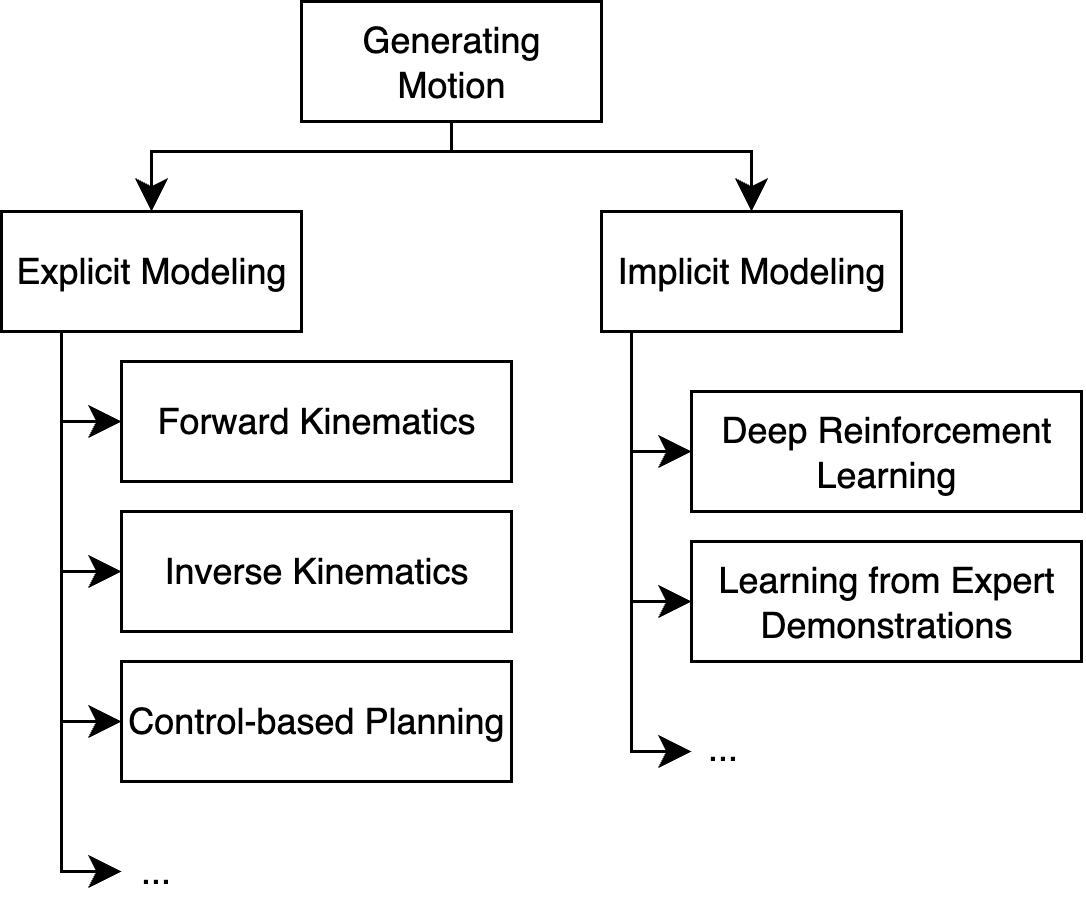
\includegraphics[width=\linewidth]{ch2/ch2-approaches.png}
    \end{column}
    \begin{column}{0.44\textwidth}
      \begin{itemize}
        \item \highlight{Explicit models}: write down mechanics, constraints, and controllers.
        \item \highlight{Implicit models}: learn motion from sensorimotor data.
        \item Real systems often mix both, but the tension between them drives modern robot learning.
      \end{itemize}
    \end{column}
  \end{columns}
  \sources{\citep{bekrisStateRobotMotion2024,hansenTemporalDifferenceLearning2022}}
\end{frame}

\begin{frame}{Robotics Is Not One Problem}
  \begin{columns}[T,onlytextwidth]
    \begin{column}{0.58\textwidth}
      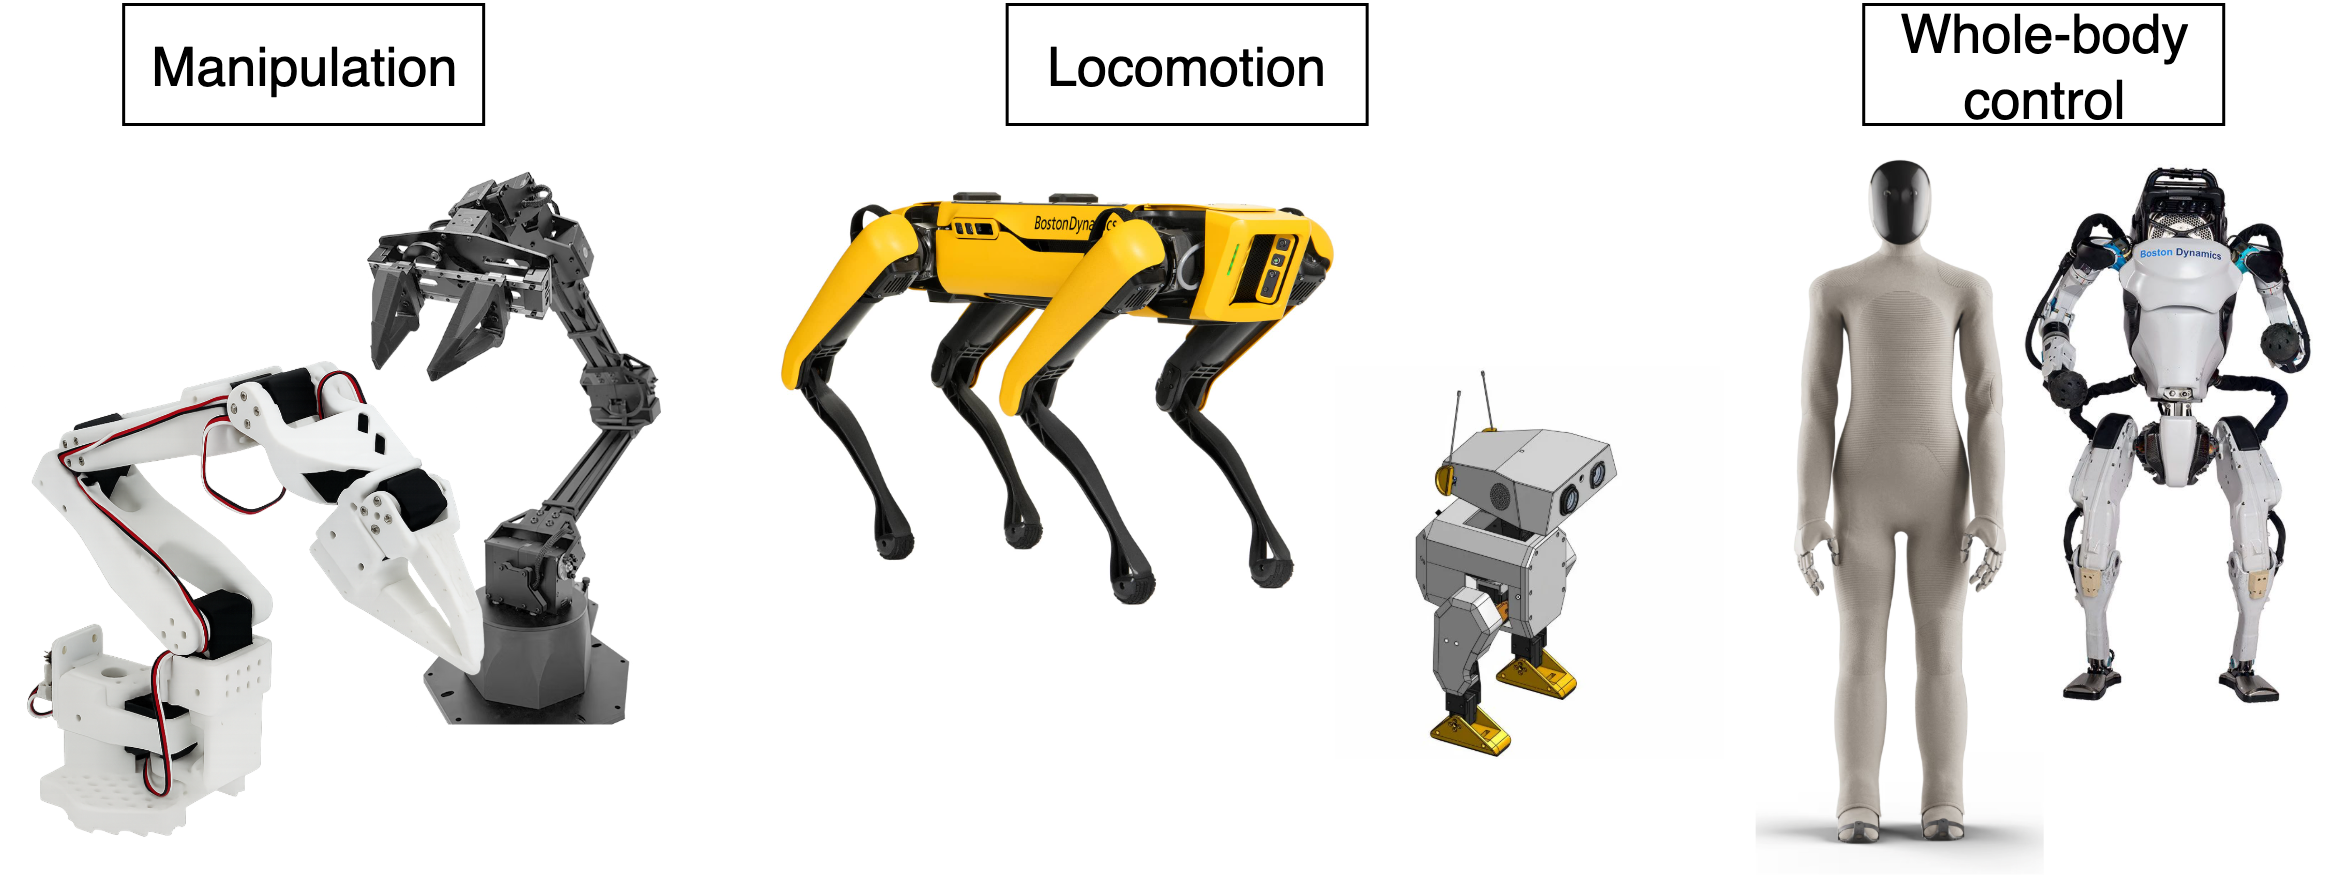
\includegraphics[width=\linewidth]{ch2/ch2-platforms.png}
    \end{column}
    \begin{column}{0.38\textwidth}
      \begin{itemize}
        \item \highlight{Manipulation}: change the environment.
        \item \highlight{Locomotion}: change the robot's position in the environment.
        \item \highlight{Mobile manipulation}: do both at once.
      \end{itemize}
    \end{column}
  \end{columns}

  \vspace{0.2cm}
  \statbox{Why this matters}{The platform, state representation, and controller design change dramatically across these settings.}
\end{frame}

\begin{frame}{A Running Example: Accessible Manipulation}
  \begin{columns}[T,onlytextwidth]
    \begin{column}{0.42\textwidth}
      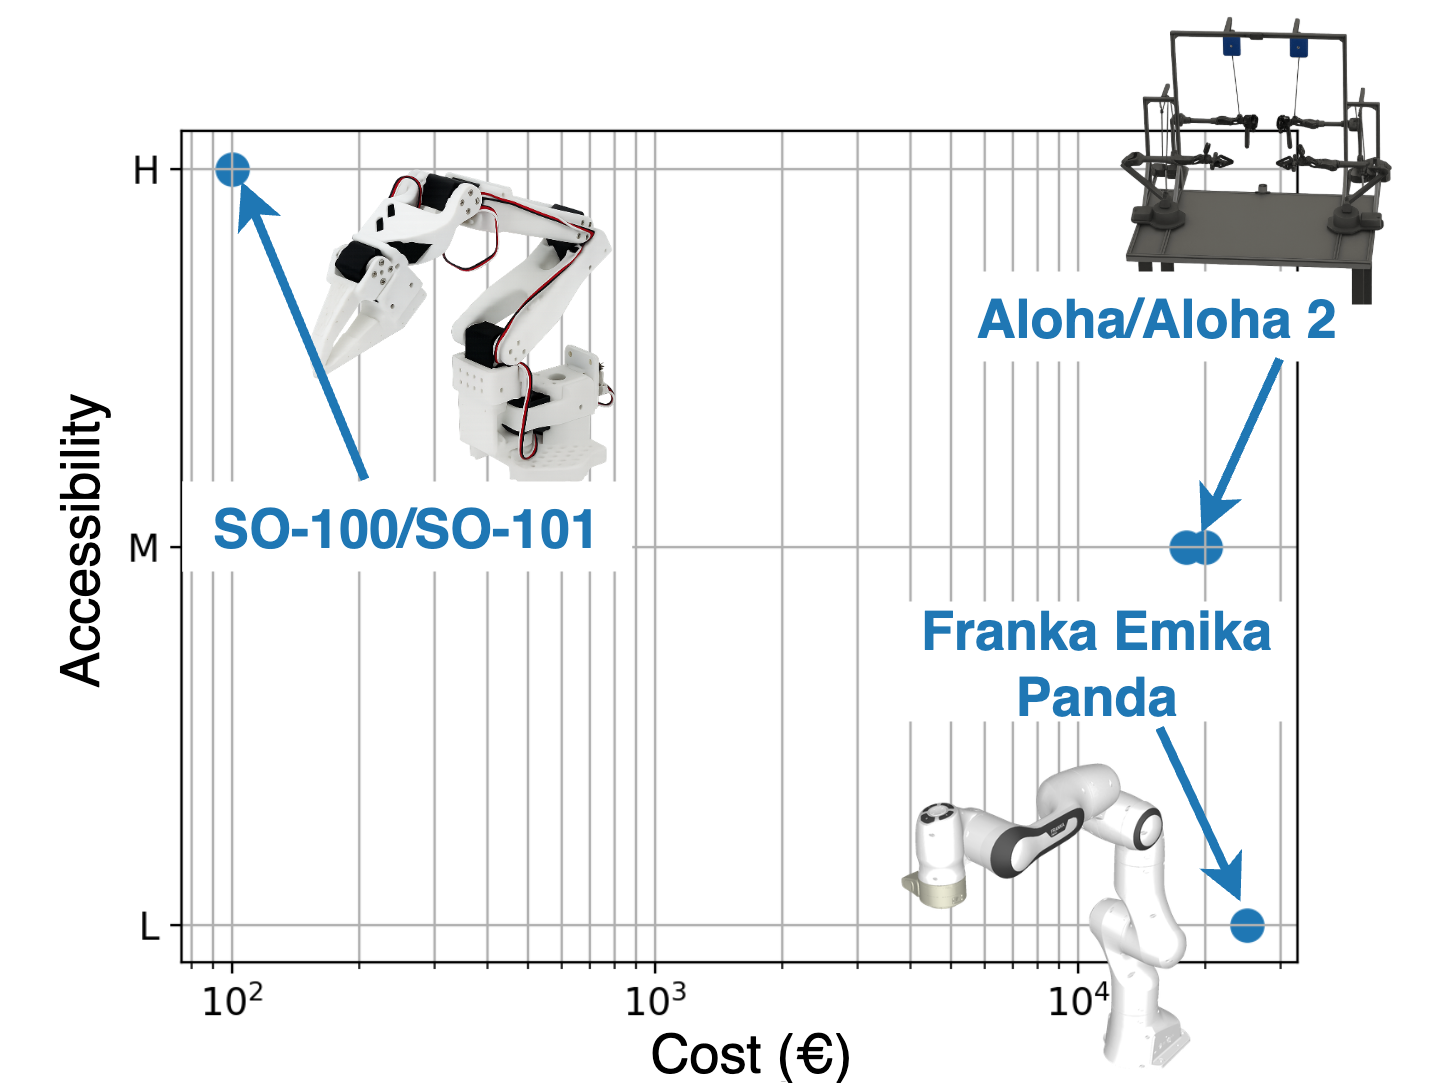
\includegraphics[width=\linewidth]{ch2/ch2-cost-accessibility.png}
    \end{column}
    \begin{column}{0.54\textwidth}
      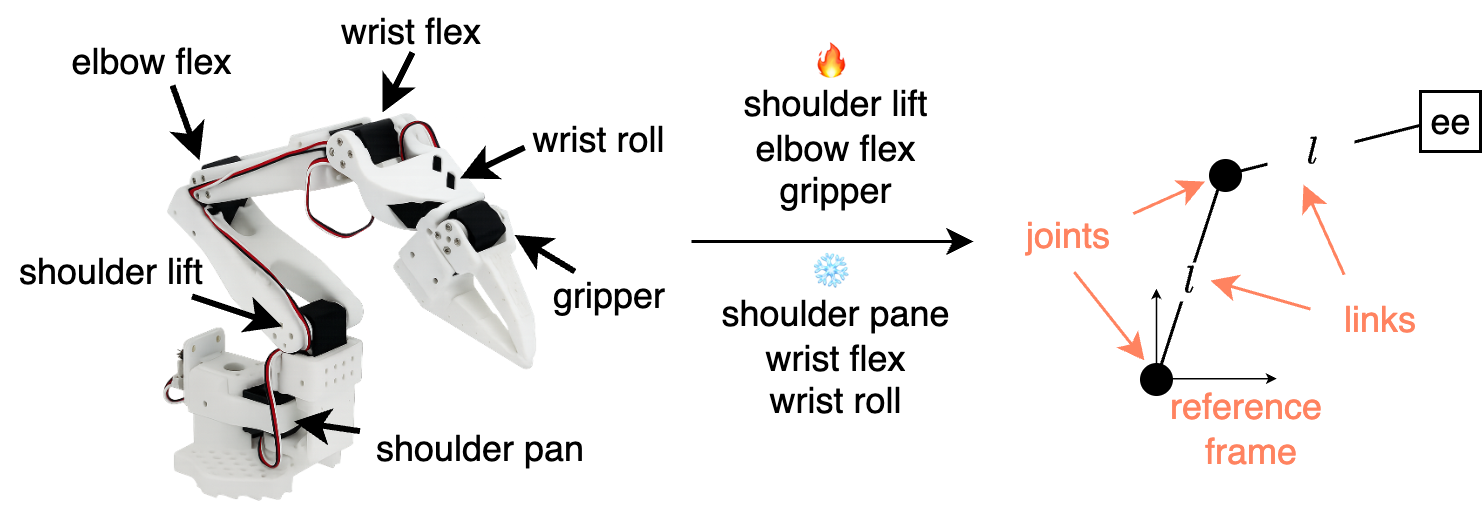
\includegraphics[width=\linewidth]{ch2/ch2-so100-to-planar-manipulator.png}
    \end{column}
  \end{columns}

  \vspace{0.2cm}
  \begin{itemize}
    \item The chapter uses a simplified planar manipulator abstraction of the SO-100 to explain core ideas.
    \item Low-cost platforms matter because they make data collection and experimentation \highlight{materially more accessible}.
  \end{itemize}
\end{frame}

\begin{frame}{From Forward Kinematics to Inverse Kinematics}
  \begin{columns}[T,onlytextwidth]
    \begin{column}{0.5\textwidth}
      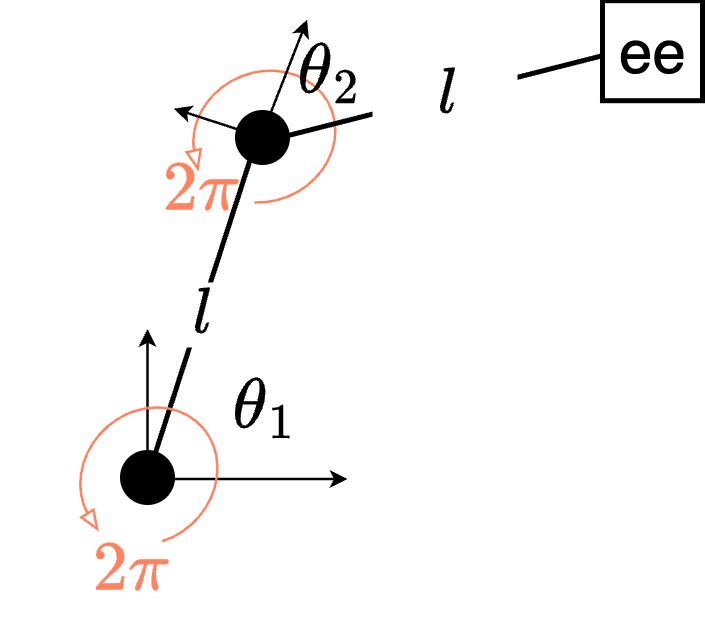
\includegraphics[width=\linewidth]{ch2/ch2-planar-manipulator-free.png}
    \end{column}
    \begin{column}{0.46\textwidth}
      \small
      \[
      p(q)=
      \begin{pmatrix}
      l\cos(\theta_1)+l\cos(\theta_1+\theta_2) \\
      l\sin(\theta_1)+l\sin(\theta_1+\theta_2)
      \end{pmatrix}
      \]
      \begin{itemize}
        \item \highlight{FK}: map configuration to end-effector pose.
        \item \highlight{IK}: solve for a configuration that reaches a target pose.
      \end{itemize}
    \end{column}
  \end{columns}

  \vspace{0.2cm}
  \statbox{Core issue}{IK tells you where to be. It does not, by itself, tell you how to move there safely over time.}
  \sources{\citep{lynchModernRoboticsMechanics2017,sicilianoSpringerHandbookRobotics2016,tedrakeRoboticManipulationPerception,tedrakeUnderactuatedRoboticsAlgorithms}}
\end{frame}

\begin{frame}{Why Differential IK Matters}
  \begin{itemize}
    \item Tracking a full trajectory with repeated IK solves can be expensive.
    \item Differential IK instead solves for \highlight{joint velocities} using the Jacobian.
  \end{itemize}

  \[
  \dot q(t)=\arg\min_{\nu}\left\lVert J(q(t))\nu-\dot p^*(t)\right\rVert_2^2
  \]

  \begin{itemize}
    \item In favorable settings this admits a closed-form pseudo-inverse solution.
    \item That makes it practical for structured, well-understood environments.
  \end{itemize}
\end{frame}

\begin{frame}{Environment Constraints Change the Problem}
  \begin{columns}[T,onlytextwidth]
    \begin{column}{0.32\textwidth}
      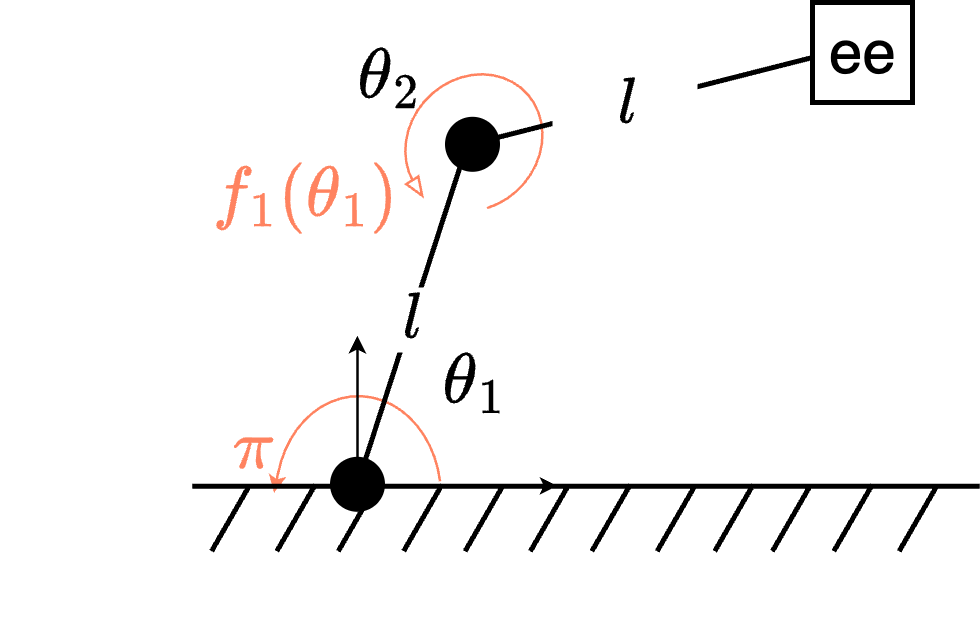
\includegraphics[width=\linewidth]{ch2/ch2-planar-manipulator-floor.png}
    \end{column}
    \begin{column}{0.32\textwidth}
      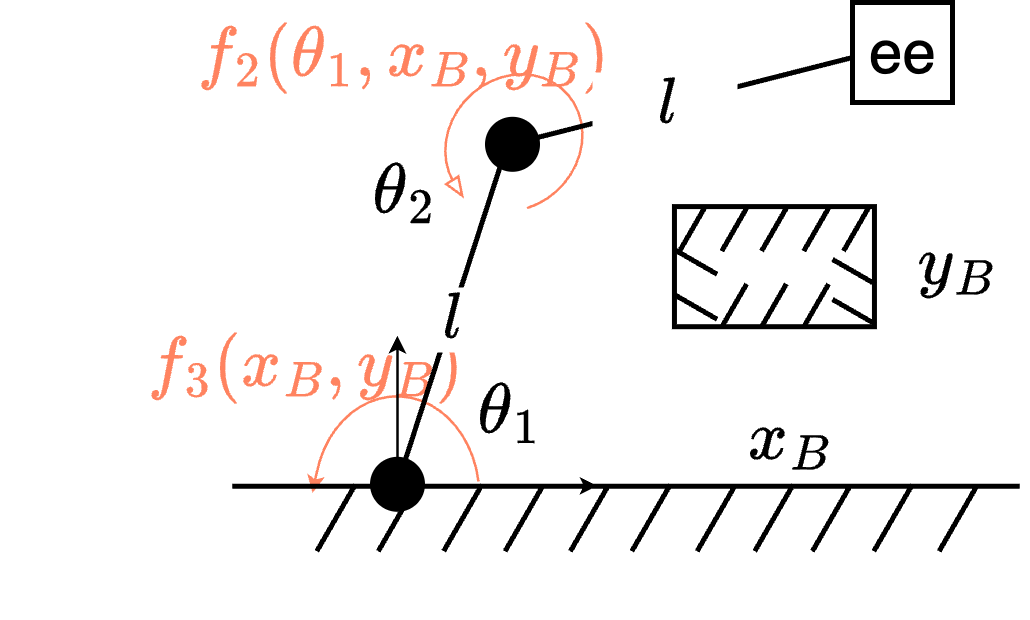
\includegraphics[width=\linewidth]{ch2/ch2-planar-manipulator-floor-shelf.png}
    \end{column}
    \begin{column}{0.32\textwidth}
      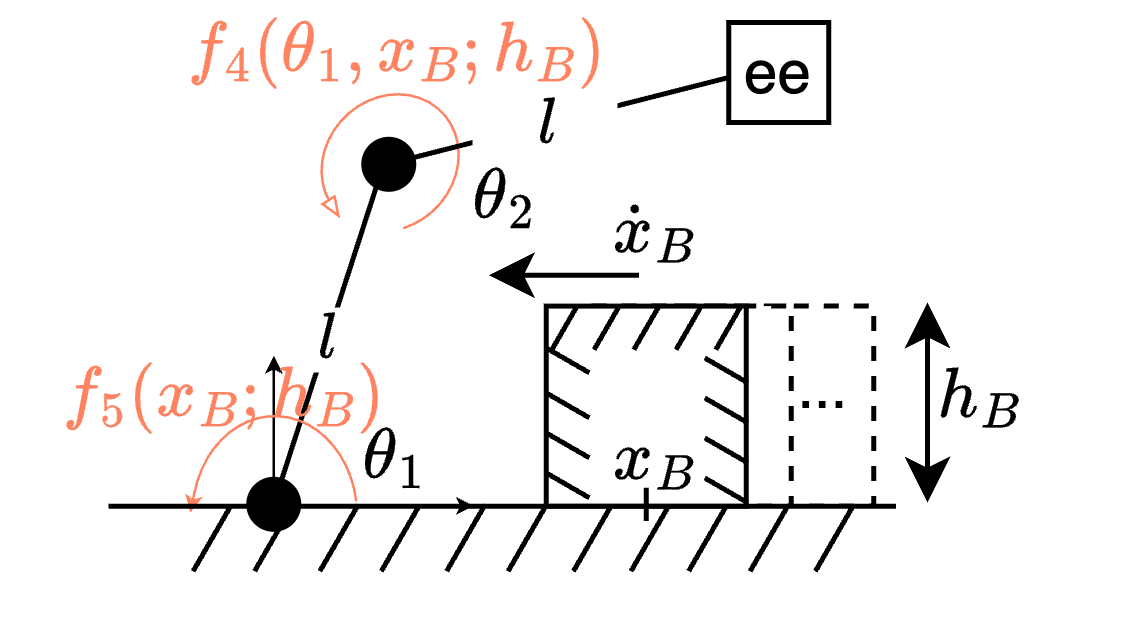
\includegraphics[width=\linewidth]{ch2/ch2-planar-manipulator-floor-box.png}
    \end{column}
  \end{columns}

  \vspace{0.25cm}
  \begin{itemize}
    \item Surfaces, shelves, and moving obstacles alter the feasible set of motions.
    \item The controller now depends on \highlight{task-specific geometry, contacts, and disturbances}.
  \end{itemize}
\end{frame}

\begin{frame}{Feedback Loops Help, but at a Price}
  \begin{itemize}
    \item Closed-loop control corrects tracking errors by feeding pose error back into the command.
    \item This improves robustness to noise and moderate perturbations.
    \item But performance still depends on:
    \item accurate sensing, gain tuning, system-specific heuristics, and manageable contact dynamics.
  \end{itemize}

  \vspace{0.25cm}
  \statbox{Practical reality}{Feedback reduces modeling error. It does not remove the need to decide what to model, how to tune it, and how to integrate many brittle components.}
\end{frame}

\begin{frame}{Where Classical Pipelines Break}
  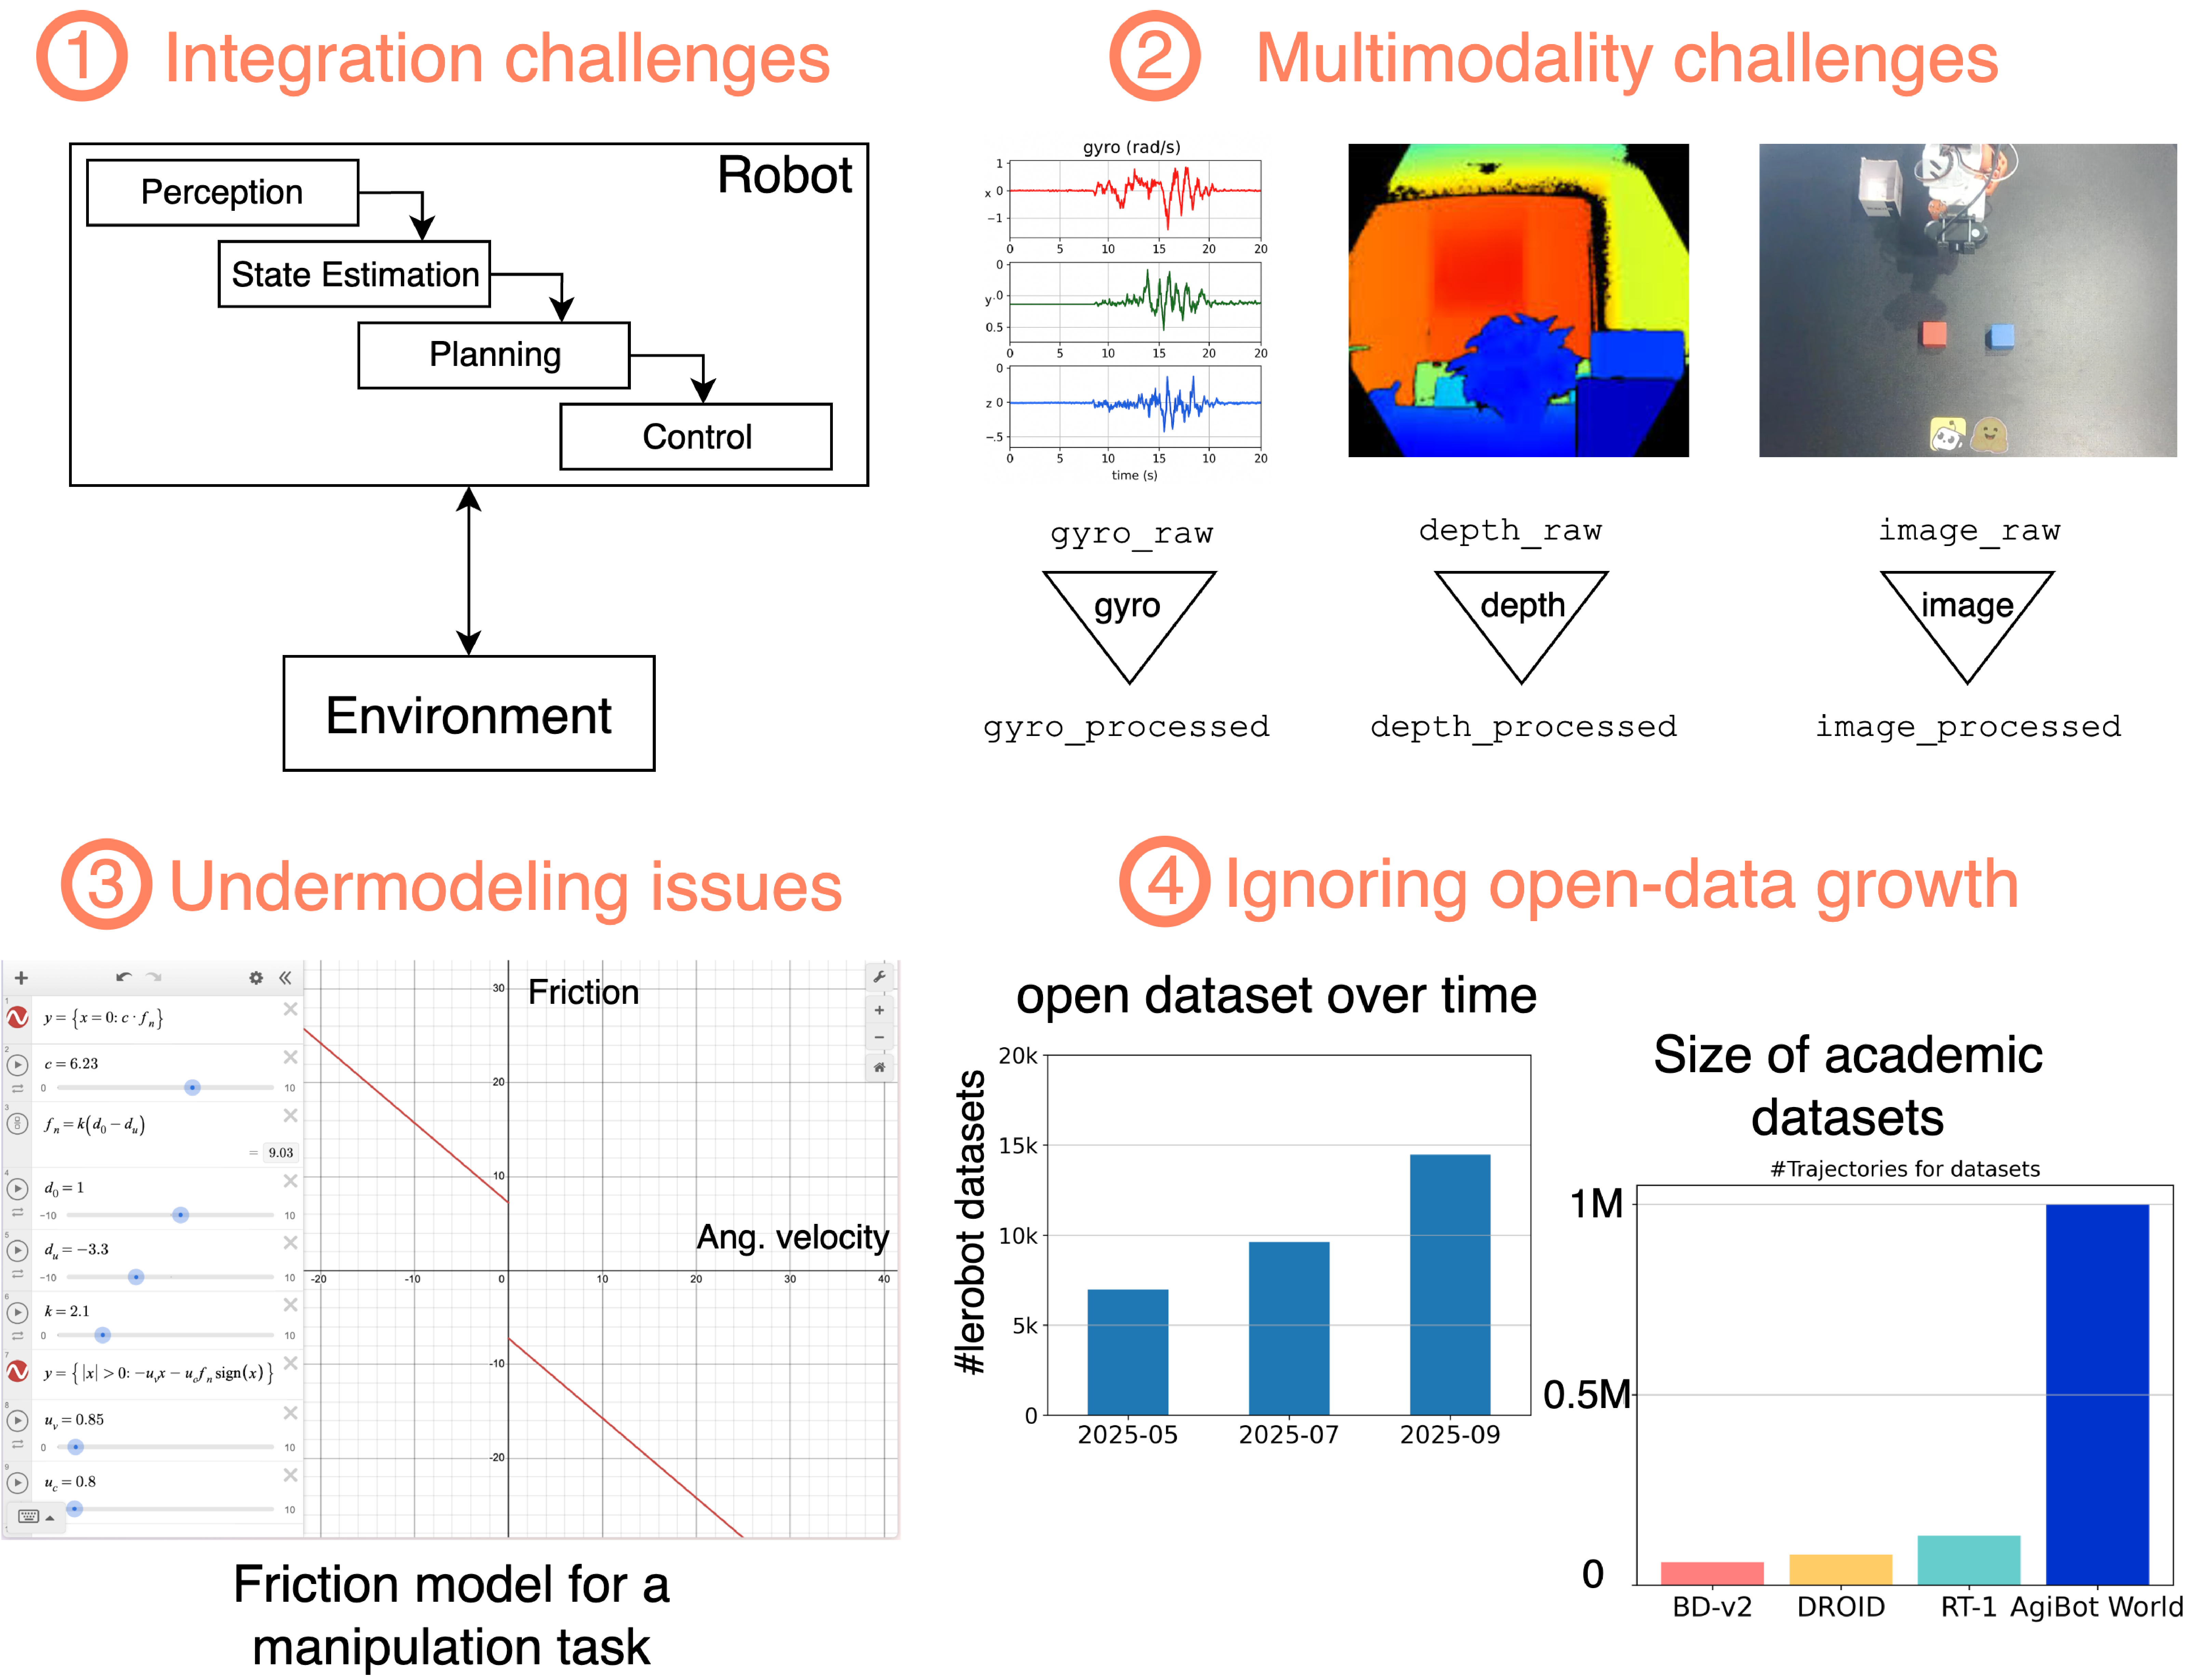
\includegraphics[width=\linewidth,height=0.68\textheight,keepaspectratio]{ch2/ch2-classical-limitations.png}
  \begin{itemize}
    \item Integration overhead, handcrafted perception pipelines, approximated physics, and weak reuse across tasks all accumulate.
  \end{itemize}
  \sources{\citep{antonovaReinforcementLearningPivoting2017}}
\end{frame}

\begin{frame}{Why Learning Becomes Attractive}
  \begin{itemize}
    \item Learn directly from high-dimensional observations instead of hand-designing every intermediate representation.
    \item Reuse data across tasks and embodiments rather than rebuilding planners and controllers for each one.
    \item Benefit from the recent surge of \highlight{open robotics datasets} rather than leaving that signal mostly unused.
  \end{itemize}

  \vspace{0.25cm}
  \statbox{Chapter takeaway}{Classical robotics gives structure, guarantees, and foundational intuition. Robot learning becomes attractive when modeling, integration, and scaling costs dominate.}
\end{frame}

\begin{frame}[allowframebreaks]{Selected References}
\scriptsize
\nocite{sicilianoSpringerHandbookRobotics2016,lynchModernRoboticsMechanics2017,tedrakeRoboticManipulationPerception,tedrakeUnderactuatedRoboticsAlgorithms,bekrisStateRobotMotion2024}
\bibliography{../shared/references}
\end{frame}

\end{document}
